%\documentclass[10pt, a4paper,english,spanish,final]{article}
\documentclass{article}

\usepackage{listings}
\usepackage{amsmath}
\usepackage{amsfonts}
\usepackage{amssymb}
\pagestyle{empty}
\usepackage{graphicx}
\usepackage{color}
\usepackage{parskip}
\usepackage{amsthm}
\usepackage{framed}

\usepackage[paper=letterpaper, left=0.5cm, right=1.5cm, bottom=1.5cm, top=2cm]{geometry}
\usepackage[T1]{fontenc}
\usepackage{indentfirst}
\usepackage{fancyhdr}
\usepackage{latexsym}
\usepackage{lastpage}
%\usepackage[colorlinks=true, linkcolor=blue]{hyperref}
\usepackage{calc}
\usepackage{algorithmic}
\usepackage{algorithm}
%\usepackage[spanish]{babel}
\usepackage[utf8]{inputenc}
\usepackage{pgf}
\usepackage{tikz}
\usetikzlibrary{arrows,automata}
\usepackage{cancel}
\renewcommand*\contentsname{\'Indice} % SI NO SE USA EL BABEL

\begin{document}

\section{Pruebas}
Para realizar los tests se realizó una base con los siguientes viajes. Para simplificar, sólo se muestra la información relevante:
\begin{center}
	

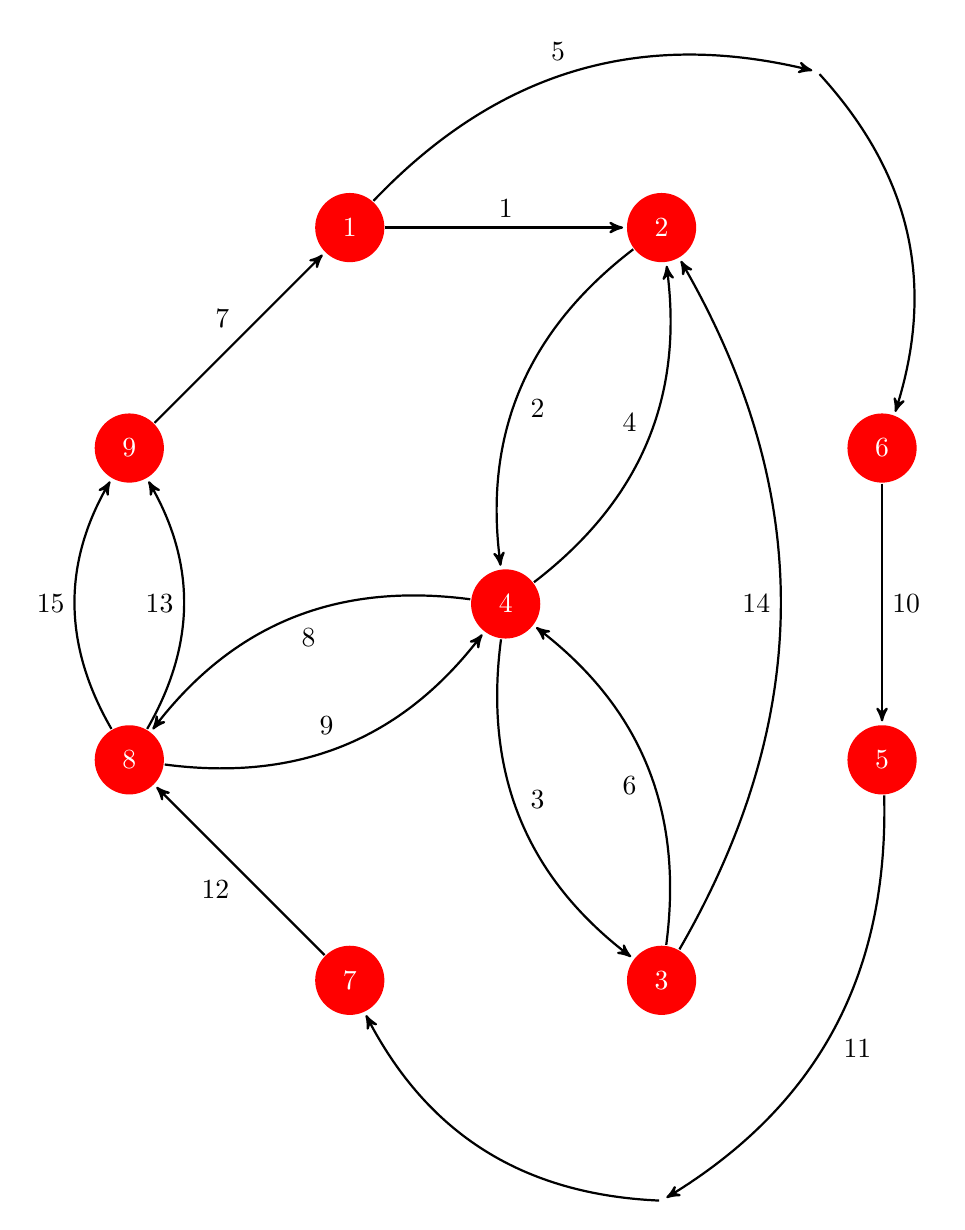
\begin{tikzpicture}[->,>=stealth',shorten >=1pt,auto,node distance=2.8cm,thick]
	\tikzstyle{every state}=[fill=red,draw=none,text=white,inner sep=2pt]

	\node[state] 		 (4)               {$4$};
	\node[fill=none,draw=none,text=white,inner sep=0pt] 		 (fi) [left of=4]  {};
	\node[fill=none,draw=none,text=white,inner sep=0pt]  		 (fd) [right of=4]  {};
	\node[fill=none,draw=none,text=white,inner sep=0pt]  		 (fu) [above of=4]  {};
	\node[fill=none,draw=none,text=white,inner sep=0pt]  		 (fa) [below of=4]  {};
	\node[state]         (1) [above left of=fu] {$1$};
	\node[state]         (2) [above right of=fu] {$2$};
	\node[state]         (3) [below right of=fa] {$3$};
	\node[state]         (5) [below right of=fd] {$5$};
	\node[state]         (6) [above right of=fd] {$6$};
	\node[state]         (7) [below left of=fa] {$7$};
	\node[state]         (8) [below left of=fi] {$8$};
	\node[state]         (9) [above left of=fi] {$9$};
	\node[fill=none,draw=none,text=white,inner sep=0pt]         (i1) [above right of=2] {};
	\node[fill=none,draw=none,text=white,inner sep=0pt]         (i2) [below of=3] {};


	\path (1) edge              node {1} (2)
	      (2) edge [bend right] node {2} (4)
	      (4) edge [bend right] node {3} (3)
	      (4) edge [bend right] node {4} (2)
	      (1) edge [bend left] node {5} (i1)
		  (i1) edge [bend left]   node {} (6)
	      (3) edge [bend right] node {6} (4)
	      (9) edge              node {7} (1)
	      (4) edge [bend right] node {8} (8)
	      (8) edge [bend right] node {9} (4)
	      (6) edge              node {10} (5)
	      (5) edge     [bend left]         node {11} (i2)
	      (i2) edge       [bend left]       node {} (7)
	      (7) edge              node {12} (8)
	      (8) edge  [bend right]  node {13} (9)
	      (3) edge  [bend right] node {14} (2)
	      (8) edge  [bend left] node {15} (9);
	% \draw[-](A) to node {2} (D);
	% \draw[-](A) to node {20} (C);
	% \draw[-](E) to node {8} (D);
\end{tikzpicture}
\end{center}



Donde los nodos representan los índices de los siguientes aeropuertos:
\begin{center}
	\begin{tabular}{ c | c | c | c}
	  \textbf{Indice} & \textbf{Aeropuerto} & \textbf{Ciudad} & \textbf{País}\\ \hline
	  1 & JFK & New York & USA \\
	  2 & LGA & New York & USA \\
	  3 & Ezeiza & Buenos Aires & Argentina\\
	  4 & Aeroparque & Buenos Aires & Argentina\\
	  5 & Heathrow & Londres & Inglaterra \\
	  6 & Pajas Blancas & Córdoba & Argentina \\
	  7 & Carrasco & Montevideo & Uruguay \\
	  8 & Doha International Airport & Doha & Quatar \\
	  9 & Guarulhos & Sao Paulo & Brasil \\
	  
	\end{tabular}	
\end{center}

A su vez, se realizaron los siguientes vuelos con escalas:
\begin{center}
	\begin{tabular}{ c | c | c }
	\textbf{Índice} & \textbf{Aeropuertos} & \textbf{Vuelos Directos} \\ \hline
	1 & 1 - 6 - 5 - 7 - 8 - 9 & 5 - 10 - 11 - 12 - 13 \\
	2 & 9 - 1 - 2 - 4 - 3 & 7 - 1 - 2 - 3 \\
	3 & 4 - 8 - 4 - 2 & 8 - 9 - 4 \\
	4 & 1 - 6 & 5 \\
	5 & 3 - 4 & 6 \\
	6 & 4 - 3 & 3 \\
	7 & 6 - 5 & 10 \\
	8 & 5 - 7 & 11 \\
	9 & 4 - 8 & 8 \\
	10 & 8 - 9 & 13 \\
	11 & 9 - 1 & 7 \\
	12 & 9 - 1 & 14 \\
	13 & 9 - 1 & 15 \\
	\end{tabular}
\end{center}


Los usuarios realizaron las siguientes reservas:
\begin{center}
	\begin{tabular}{ c | c | c }
	\textbf{idUsuario} & \textbf{Nombre} & \textbf{idVueloConEscala} \\ \hline
		8 & Federico & 4 \\
		8 & Federico & 8 \\
		8 & Federico & 10 \\
		8 & Federico & 9 \\
		8 & Federico & 7 \\
		8 & Federico & 11 \\
		7 & Vanesa & 4 \\
		3 & Pablo & 1 \\
		2 & Manu & 5 \\
		1 & Juampi & 3 \\
		6 & Matías & 2 \\
	\end{tabular}
\end{center}

La consulta SQL del ejercicio 5, modificada de la siguiente forma para claridad de resultados:
\begin{align*}
	& \text{\texttt{SELECT} aeropuerto, \texttt{SUM}(entrada), \texttt{SUM}(salida)} \\
	& \text{\texttt{FROM} resultado\_ejercicio\_5} \\
	& \text{\texttt{GROUP BY} aeropuerto} \\
\end{align*}

Debería dar la siguiente tabla:
\begin{center}
	\begin{tabular}{ c | c | c}
		\textbf{Aeropuerto} & \textbf{Entrada} & \textbf{Salida} \\ \hline
		1 & 2 & 4 \\
		2 & 2 & 1 \\
		3 & 1 & 1 \\
		4 & 3 & 3 \\
		5 & 2 & 2 \\
		6 & 3 & 2 \\
		7 & 2 & 1 \\
		8 & 3 & 3 \\
		9 & 2 & 2 \\
	\end{tabular}
\end{center}

\end{document}
